\section{Lista dei bug}
\subsection{Reset dei filtri}
\textbf{Stato:} risolto\\
Nella prima implementazione, il reset del filtro per valore del dataset,
attivato selezionando una barra del grafico o una cella della tabella,
non riportava tutte le barre al loro stato originale: la barra che era
stata selezionata manteneva il colore di selezione.

\subsection{Opacità delle barre}
\textbf{Stato:} risolto\\
Inizialmente, ogni barra del grafico era rappresentata da una mesh, ciascuna
con il proprio materiale, il che portava a un numero eccessivo di draw call e
dunque a un rallentamento delle prestazioni. 
Per risolvere questo problema, è stata usata la classe Instanced Mesh, che consente di
raggruppare più mesh in un'unica mesh, riducendo il numero di draw call.
Il problema è che tutte le mesh condividono lo stesso materiale, il che rende
impossibile modificare l'opacità di una singola barra. Per questo motivo,
è stato necessario implementare un sistema di shader personalizzati, passando
in ingresso un array di opacità per ogni barra. In questo modo, si può
modificare l'opacità di ogni barra in modo indipendente, senza influenzare le altre.

\subsection{Trasparenza delle barre}
\textbf{Stato:} non risolto\\
Come noto, in caso di filtraggio del dataset, le barre del grafico
che non soddisfano i criteri di selezione vengono rese trasparenti.
È lecito aspettarsi che, se due barre sono sovrapposte e la barra più vicina all'osservatore
è trasparente, la barra più lontana sia visibile. Tuttavia, in alcuni casi,
una barra trasparente può nascondere completamente una barra più lontana.
In figura \ref{fig:trasparenza} sono mostrati due esempi di barre trasparenti.
A sinistra, la barra più vicina è trasparente e non nasconde
completamente la barra più lontana (comportamento atteso). A destra, invece,
la barra più vicina è trasparente e nasconde completamente la barra 
più lontana (comportamento ottenuto in certi casi).
\begin{figure}[h!]
    \centering
    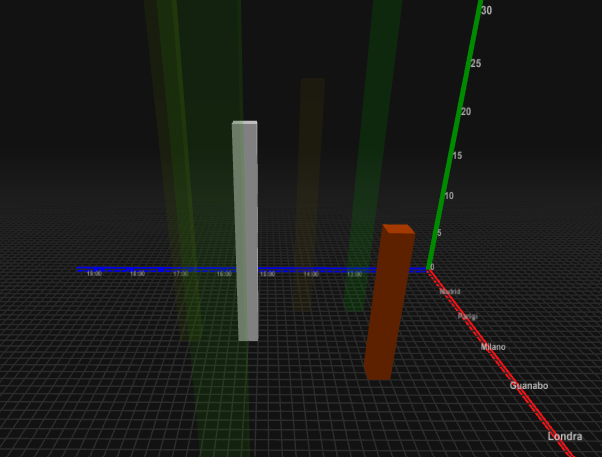
\includegraphics[width=0.4\textwidth]{template/images/barreok.png}
    \hspace{0.5cm}
    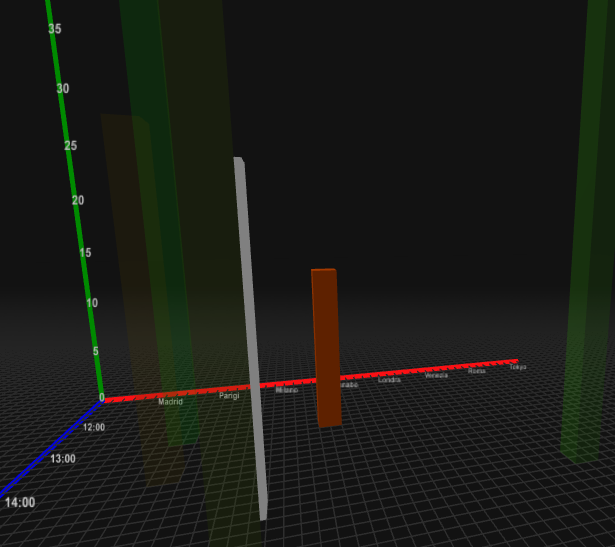
\includegraphics[width=0.4\textwidth]{template/images/barre.png}
    \caption{Esempio di barre trasparenti}
    \label{fig:trasparenza}
\end{figure}

\subsection{Rotazione del grafico}
\textbf{Stato:} non risolto\\
La rotazione del grafico avviene in modo fluido e senza evidenti problemi. Tuttavia,
se nella posizione iniziale il cursore del mouse si trova sopra una barra, e
nella nuova posizione il cursore si trova sopra un'altra (o la stessa) barra,
quest'ultima viene selezionata al momento del rilascio del mouse.
Questo comportamento è strettamente legato alla
gestione dell'evento "onClick" del mesh, che viene attivato al momento del rilascio del tasto sinistro del mouse.